\documentclass[12pt,fleqn,a4paper]{article}

\usepackage{latexsym}
\usepackage{url}
\usepackage{xspace}
\usepackage{epsfig}
\usepackage{psfrag}
\usepackage{a4wide}
\usepackage{marvosym}
\usepackage{amsmath,amsfonts,amssymb,amsthm,latexsym}
\usepackage{graphics,graphicx,color,subfigure}
\usepackage{fancyhdr}
\usepackage[english]{babel}
\usepackage[latin1]{inputenc}
\usepackage{listings}

\textheight 680pt
\textwidth 460pt
\topmargin -40pt
\oddsidemargin 5pt
\evensidemargin 5pt
\parindent 0pt

\pagestyle{fancyplain} \setlength{\headheight}{16pt}
\renewcommand{\sectionmark}[1]{\markright{\thesection\ #1}}
\lhead[\fancyplain{}{\thepage}]
    {\fancyplain{}{\rightmark}}
\rhead[\fancyplain{}{\leftmark}]
    {\fancyplain{}{\thepage}}
\cfoot{}
\renewcommand{\thesection}{\arabic{section}}
\renewcommand{\thesubsection}{\arabic{section}.\arabic{subsection}}


\begin{document}
\begin{titlepage}%Institution
\vspace{2cm}
\centerline{
\large{Department of Computer Sciences}}
\vspace{0.2cm}
\centerline{\large{University of Salzburg}}%Title with one or two Lines(More if wanted)
%\hline
\vspace{2cm}

\centerline{\large{PS Natural Computation}}
\centerline{SS 15/16}
\vspace{1cm}

\centerline{\Large{\bf{Evolution of a Poker Player Using Genetic Programming}} }%Type of the Document
\vspace{1cm}

\vspace{0.4cm}%Date
\centerline{\today}
\vspace{4.5cm}%Authors

%\hline
\vspace{0.2cm}
Project Members:\\
\centerline{Thomas Samy Dafir, 1331483, tdafir@cosy.sbg.ac.at}\\
\centerline{Laurentiu Vlad, 1423336, lvlad@cosy.sbg.ac.at}\\
\centerline{Dominik Baumgartner, 0920177, dbaumgart@cosy.sbg.ac.at}\\
\centerline{Sebastian Strumegger, 1420277, sstrumegg@cosy.sbg.ac.at}\\
\vspace {1cm}\\

Academic Supervisor: \\
\centerline{Helmut MAYER}
\centerline{helmut@cosy.sbg.ac.at}
\vspace{1.5cm}\\
Correspondence to: \\
\centerline{Universit\"{a}t Salzburg} \\
\centerline{Fachbereich Computerwissenschaften} \\
\centerline{Jakob--Haringer--Stra\ss e 2} \\
\centerline{A--5020 Salzburg} \\
\centerline{Austria}
\clearpage
\end{titlepage}

%Table of Content
\setcounter{page}{1}
\pagenumbering{Roman} %I,II,III... in the TOC
\tableofcontents

\clearpage
\pagestyle{headings}
\pagenumbering{arabic}  %Better if TOC is variable (more than one page)
\setcounter{page}{1}
\pagenumbering{arabic}  %Better if TOC is variable (more than one page)
\setcounter{page}{1}

\abstract{
The goal of this project is to evolve a GP poker player by means of genetic programming techniques.
The GP Players evolve over generations through selection, mutation and cross mutation of their chromosome tree. \\
A good computer player has to emerge after a sufficient amount of generations have played in a "heads up" texas-hold-em no limit poker game.
Good players are determined by their fitness value which is determined through assessing a player's success after each poker round. \\
The focus of our work lies on the chromosome tree.
Although the current API provides some basics functions for that tree, it is likely that they are not sufficient for the evolution of a good player.
Further focus lies on the poker game itself.
We have to determine what kind of and how much information a player needs in order to evolve properly without interfering with its evolution.
This means, that we don't want to "tell" the player what the next best action is, but rather let evolution decide.
Additionally we will do some fine-tuning of evolutionary-parameters like population size or number of generations to achieve the best possible result.
}

\newpage

%\input{gp.tex}

\newpage

\section{Frameworks}
This project requires the use and interaction of two frameworks, namely GPoker and JEvolution. In the following, both frameworks and their interaction with one another will be briefly explained.

\subsection{JEvolution}
JEvolution is the most essential part of this project. JEvolution provides functionality for Evolutionary Computation including Evolutionary Algorithms and Genetic Programming which is
used in this project. JEvolution completely implements the evolution of syntax trees including selection, mutation and crossover. Syntax trees are made up from objects of type
$ProgramNode$. Each node includes an array containing all child nodes. In order for evolution to work, a set of function- and terminal-nodes has to be provided. These
are implemented as subclasses of the $ProgramNode$ class. Selection is conducted based on the computed fitness of every syntax tree. For our application of the framework,
nodes are provided by the GPoker framework and by us. In order for JEvolution to conduct evolution correctly, a function calculating a tree's fitness has to be supplied (fitness function). In
our case this function has to somehow compute how good a syntax tree (here: representing a poker player) is able to complete the given task (in this case: play poker and win
chips). Details about Genetic Programming are supplied in chapter \ref{sec:genprog}.

\subsection{GPoker}
GPoker is a poker-framework by Helmut A. Mayer. It provides a set of classes implementing a working poker setup including several game modes, different players and the
possibility for a human player to play against computer players. The most essential functionality for our application is the possibility to include evolved players and hence
use the framework to do genetic programming. GPoker provides nodes which are subclasses of the JEvolution $ProgramNode$ class representing decisions, actions and queries a
poker player might perform. Parameters like game-mode, competing players, big/small blind and rounds to play can be specified in the gpoker.xml file.

\subsection{Interaction}
How does the interaction of these two frameworks enable us to evolve a poker player?  \\
JEvolution evolves syntax trees made up from $ProgramNode$ objects. It does not care about what the functionality of a node is. As long
as it is specified as a subclass of $ProgramNode$ it can be used in a syntax tree.
Once GPoker detects that a GPlayer (evolved player) is specified in the gpoker.xml file, it communicates with JEvolution to invoke the evolutionary process.  GPoker provides nodes 
for constructing syntax trees. JEvolution then builds and evolves these trees made up from the supplied nodes. A vital component of the evolutionary process is the calculation of the fitness value. In the case
of the evolution of a poker player the fitness value should of course reflect the player's skill. The most intuitive way of defining a player's skill is measuring the amount of won/lost chips.
This value can be determined by letting the player play games of poker against other players and is then recorded as the player's fitness. JEvolution can then execute the selection part
of the evolutionary process using this fitness value provided by GPoker.
\\
Interactions can be summarized as follows :
\begin{itemize}
	\item GPoker detects an evolved player in the xml file and invokes JEvolution, providing poker specific nodes.
	\item JEvolution builds syntax trees and uses GPoker to calculate fitness values of individual syntax trees.
\end{itemize}

\newpage
\section{Genetic Programming}
\label{sec:genprog}
As mentioned, a GP Player is represented by a so-called chromosome tree. Or more precisely, the poker player's strategy is represented by this tree.\\
This means, that each player's tree has a root node and zero or more child nodes, where nodes with children are called functions and leaf nodes are called terminals.\\
From the very beginning there is a fixed set of functions and terminals available.
At first, a population of GP Players with random nodes are created which play a predetermined number of games.
In each generation there is a probability for every player to get it's tree changed by mutation or crossover.

\subsection{Chromosome Tree}
\subsubsection{Functions}
Functions play the most important role in a GP Player's strategy, since functions are the decision-makers.\\
They can have one or more child nodes and a specific return type. Further all nodes (except the root)  need to have a parent node.
Child nodes can either be terminals or functions. It is vital that the child nodes return the very type the function expects.\\
As an example we could define a lower-than function that expects floating point values from both children and returns a boolean value to it's parent node.

\subsubsection{Terminals}
Terminals are the leaf nodes in a player's tree. They cannot have child nodes but return a certain type themselves.\\
This does not necessarily mean that a terminal's value has to be static. They can have dynamic values like "pot size" or "higher hand card".

\subsubsection{Root}
The root node is a special function, since it does not have any parent nodes.\\
For proper evaluation of the player's tree it needs to be rooted, so we can start making further decisions at one point.
For GPoker we need to have a root node that always returns a poker move which is returned to the game.\\
~\\
A GPlayer, for example, uses the root node "IfMove" which has three children:\\
The very left child is the if-condition, that needs to return a boolean type.\\
The middle child is the then-branch and returns a move.\\
And at last, the right child represents the else-branch, which also returns a move.\\

\newpage

\subsubsection{Example}
\begin{center}
	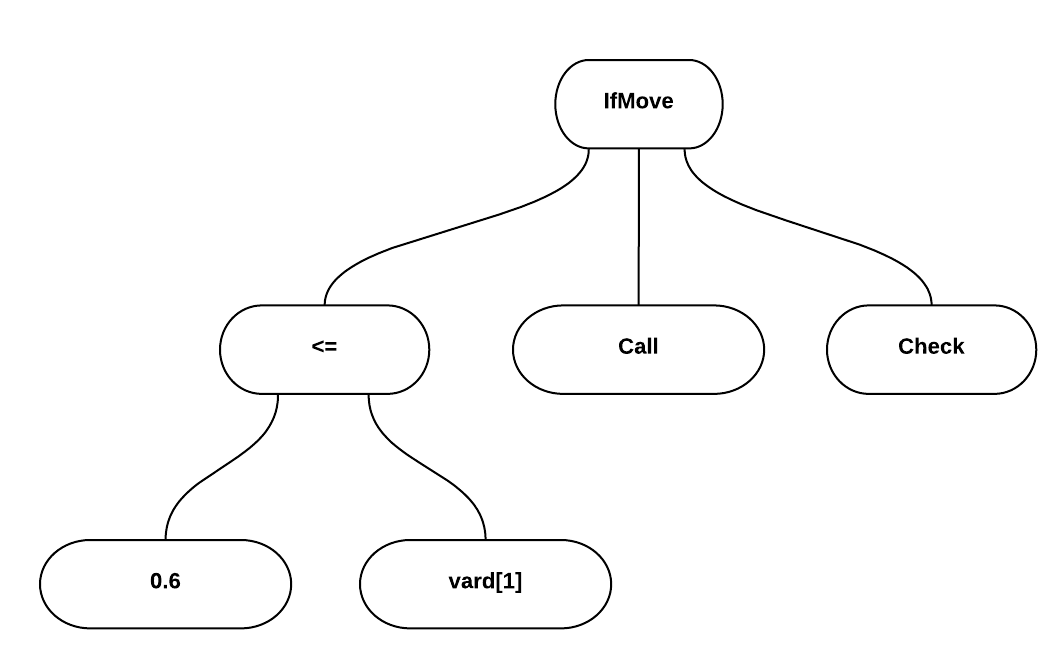
\includegraphics[width=0.8\textwidth]{tree1.png}
\end{center}
This very simple tree represents the following strategy:
~\\
If 0.6 (Two to Ace normalized in 0 to 1) is less than or equal to the player's lower hand card, make a call.\\
Else: check. Note that checking can also mean folding, in case there has been a raise.

\subsection{Evolution}
There are two fundamentally different ways for evolution to change a tree, namely crossover and mutation.

\subsubsection{Crossover}
Crossover takes two individual players and swaps subtrees in a random point.
Of course both subtrees need to have the same return type.
This method is more common, since good players that were not sorted out by evolution usually have good subtrees.
So the the well-playing trees are not completely destroyed by the process of evolution, but there is much room for new combinations.

\begin{center}
	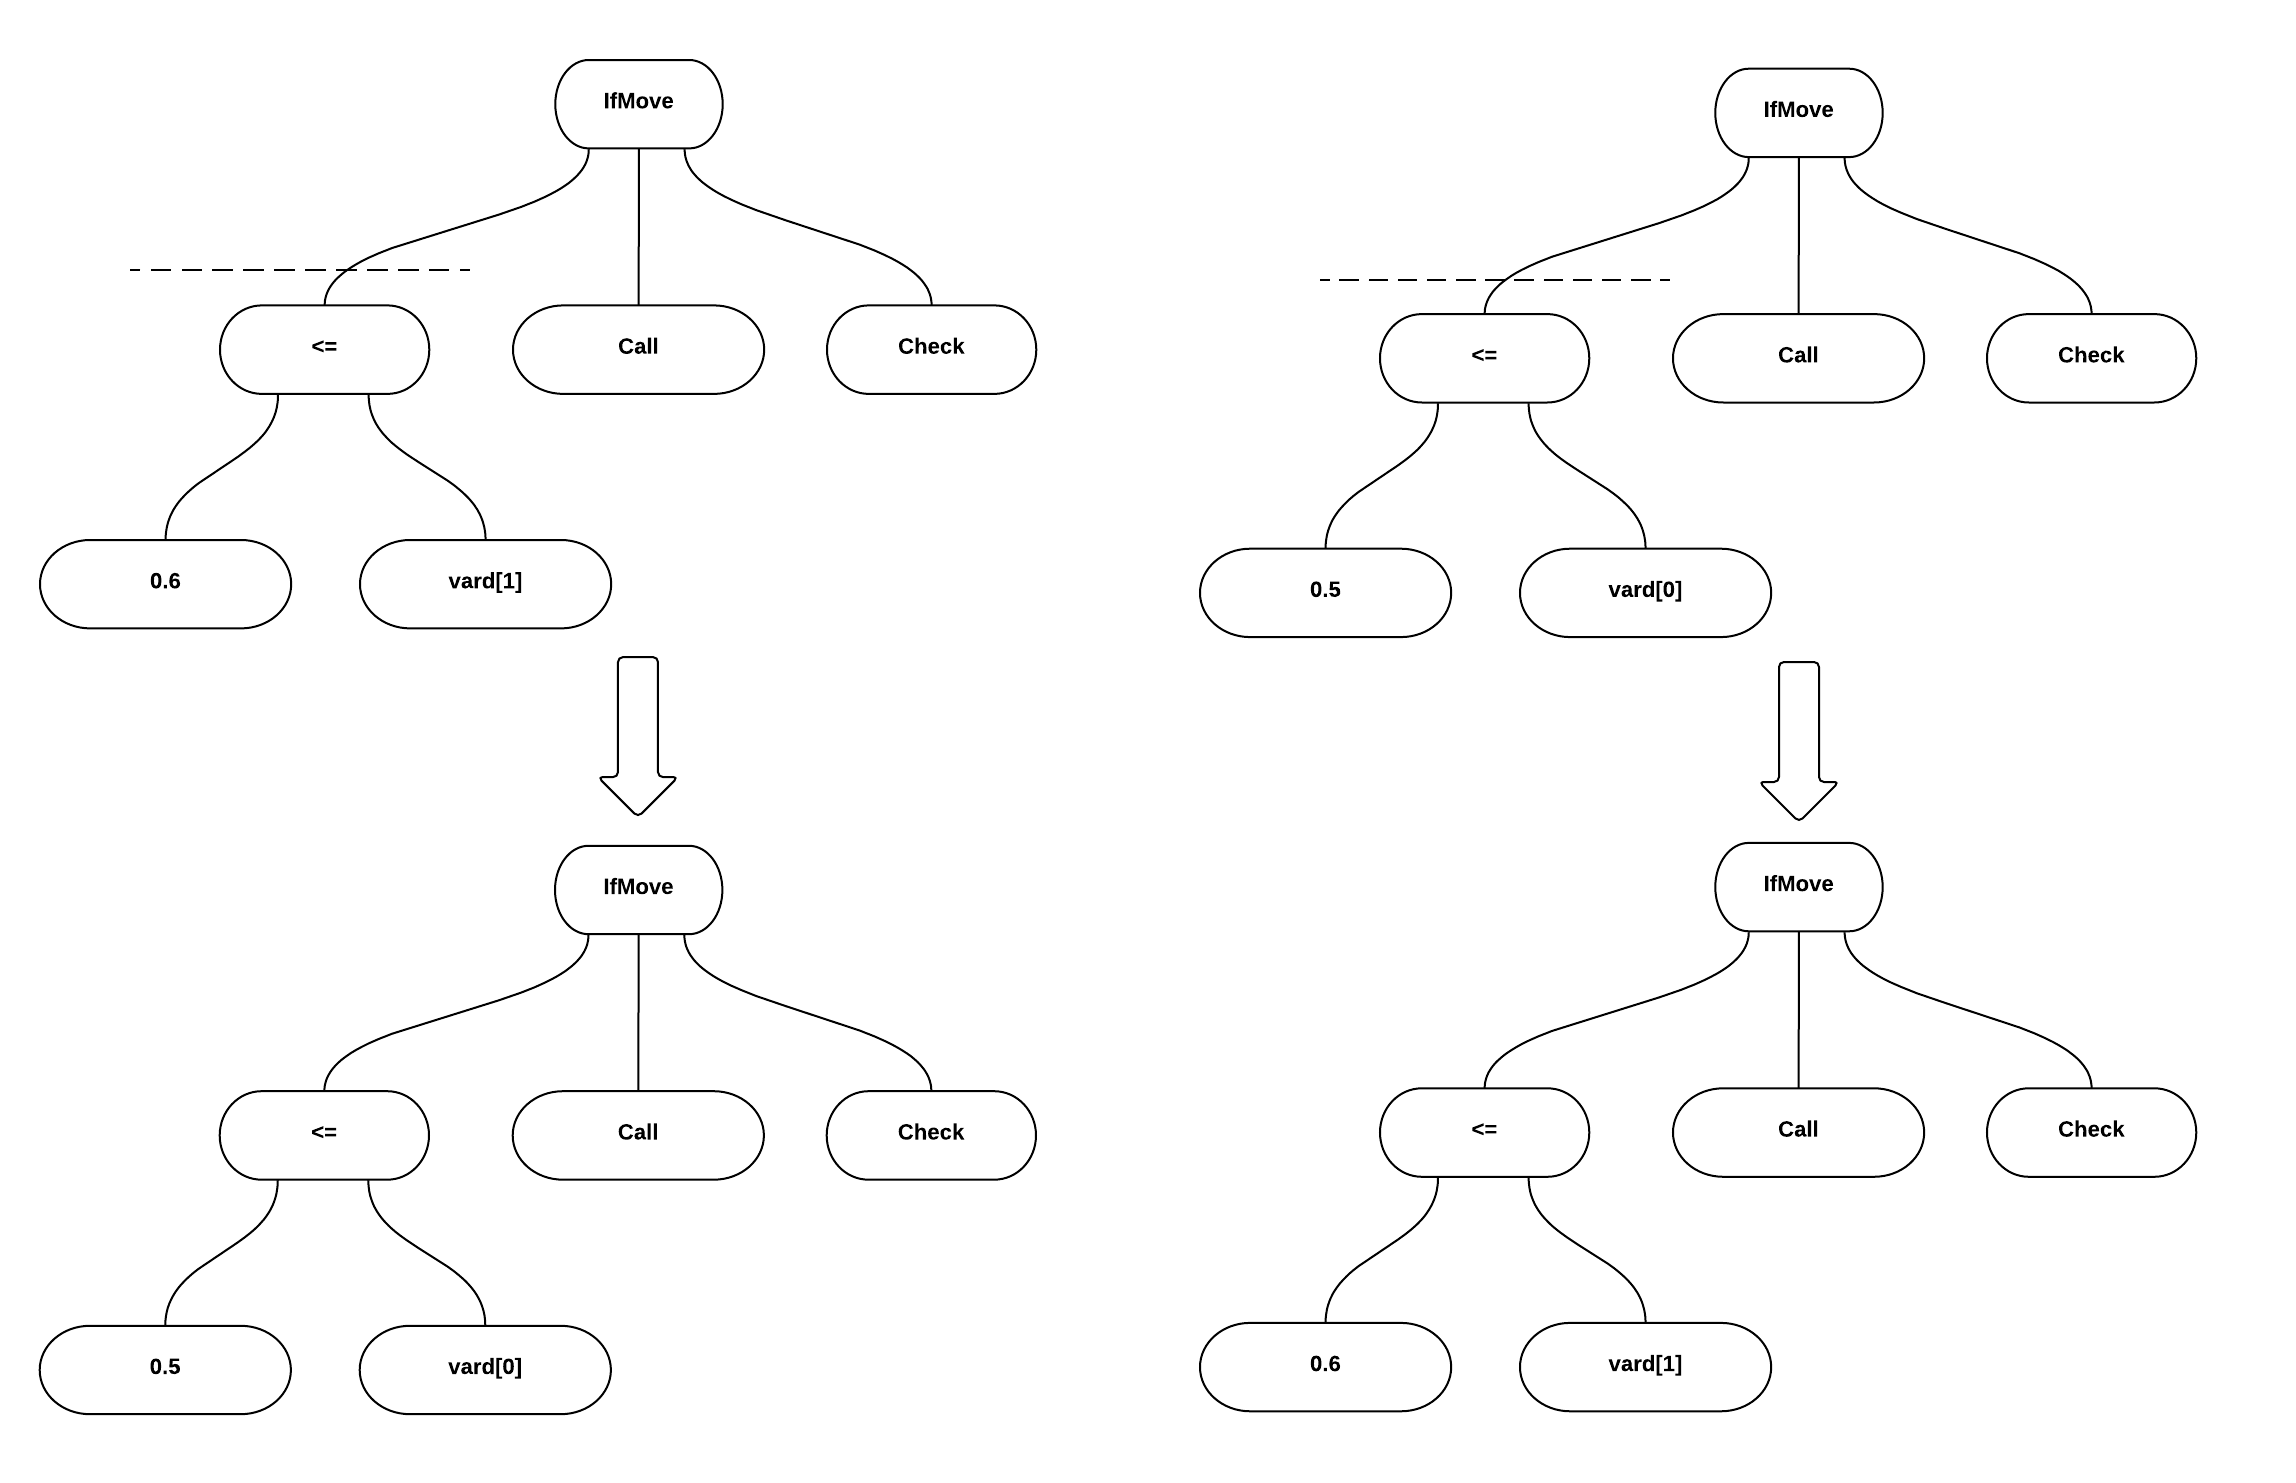
\includegraphics[width=1.0\textwidth]{tree_crossover.png}
\end{center}

\subsubsection{Mutation}
In contrast to crossover, mutation does not require two individual trees to operate.
Either a single node is chosen at random and changed to some other random node with the same return type,
or a randomly chosen subtree is modified.
Mutation has to be used carefully, since random changes can render a very good player useless.

\begin{center}
	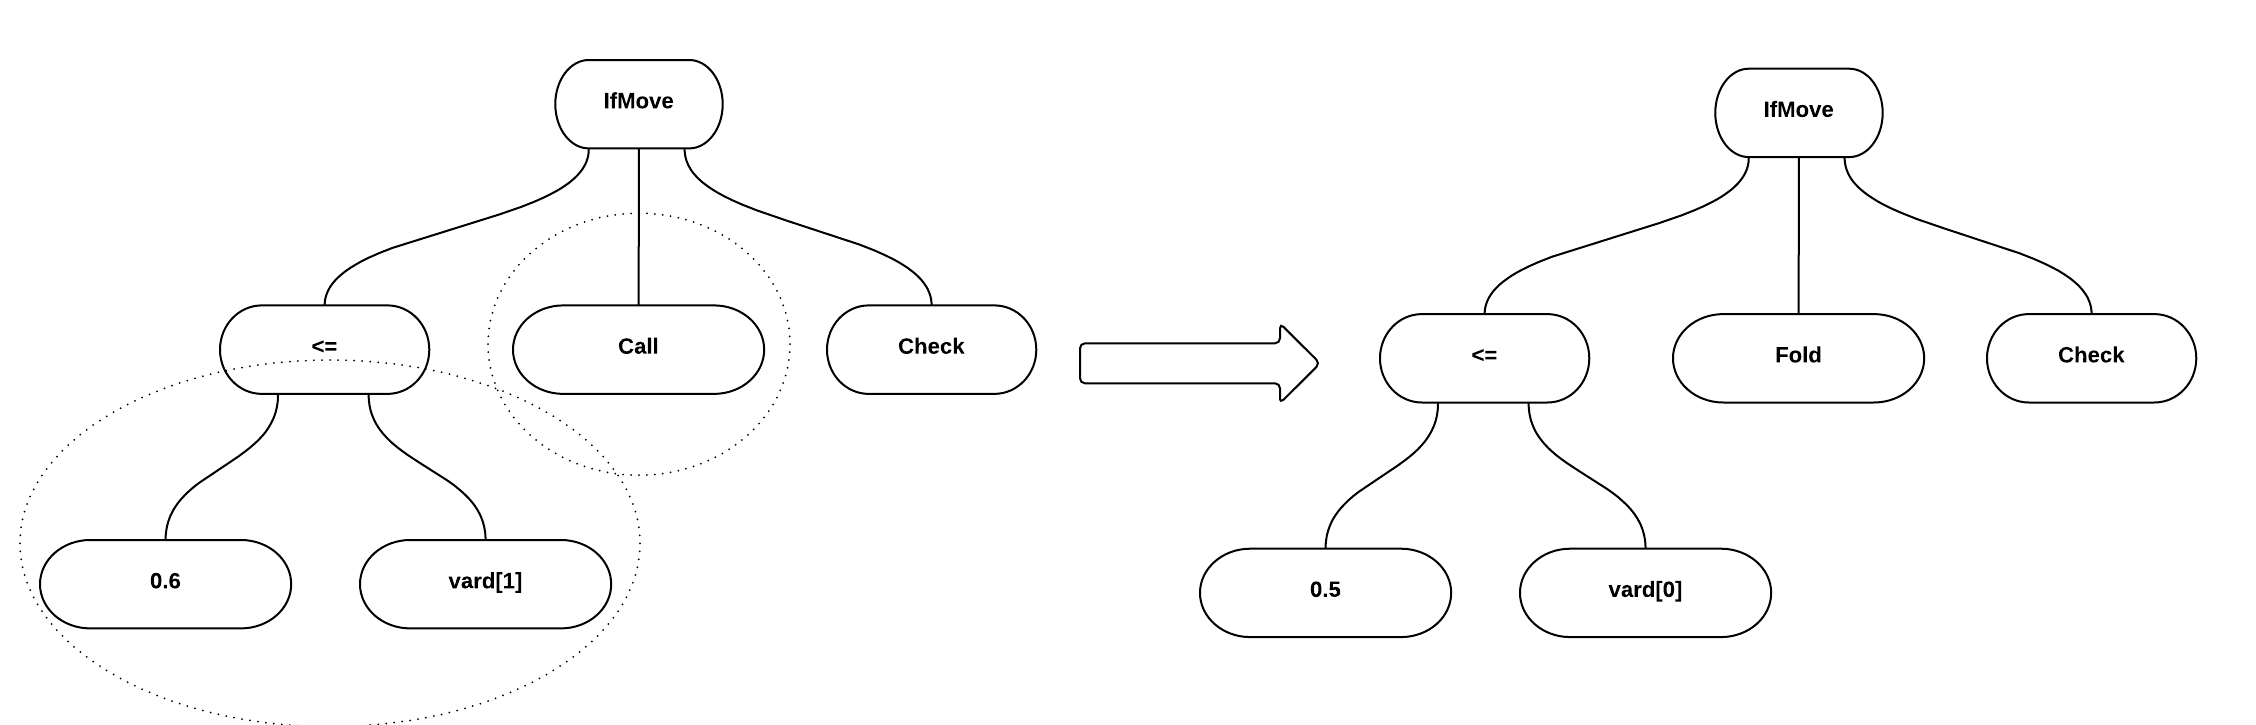
\includegraphics[width=1.0\textwidth]{tree_mutation.png}
\end{center}

\newpage
\section{Implementation}
\subsection{Initial changes}
As mentioned above, our focus in this work was to change existing nodes and/or add
new nodes to the chromosome tree. When we first evaluated the existing code, especially the implemented functions and terminals, we observed that the raise value was randomly calculated [0.0 to 2.0 * pot]. The value was neither decided nor influenced by evolution. \\
Raising plays a vital role in a Texas Hold'em No Limit poker game and this was also noticed by the evolution which often returned players who's trees were but a single raise node.
Therefore we decided to concentrate on making the raise node accessible to the evolution so its value can be evolved.
\\ \\ 
The first attempt was to allow the raise leaf-node to have a subtree which would potentially get evolved. For this purpose we introduced a new function node called "IfDouble". It evaluates a boolean expression and returns a double value which is the factor of the raise [i.e 1,9397 * pot size]. In this case, a ConstMove terminal could either be a terminal or a function node.

\begin{center}
	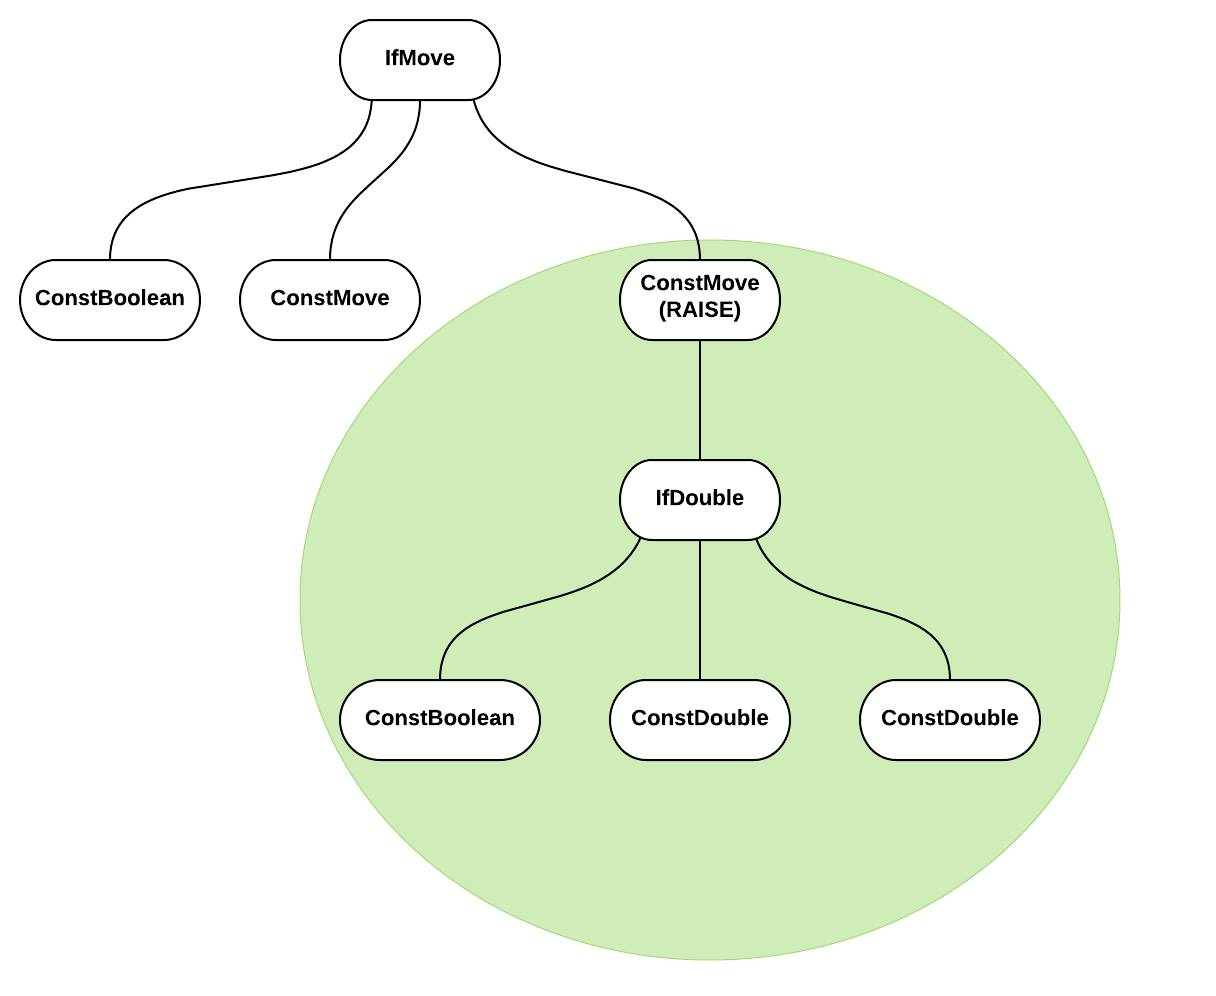
\includegraphics[width=0.86\textwidth]{raise_subtree_1.png}
	\textit{\textbf{Figure 1: }Example tree of an evolved player with an IfDouble-subtree appended to raise}
\end{center}

This however led to undesirable mutations like the following:
\begin{itemize}
	\item GPoker produced IfDouble-Nodes that only have one child
	(ConstBoolean).
	\item GPoker produced ConstMove(RAISE) Nodes that have a
	ConstDouble child which does not get evaluated.
\end{itemize}

\newpage
\subsection{Final implementation}
\subsubsection{Raise}
As a final solution, the raise move was moved out of ConstMove and implemented as an independent function node. It still has only one child but now the lines between functions and terminals are no longer blurred. With this change, the evolution can now remove raise entirely if it finds that it is not a good function. Additionally, it is now easier to mutate the factor of a raise which is more dynamic and granular. \\
This is due to a raise subtree now being able to grow or shrink and build up different calculations for the raise factor like multiplying the high card with another factor. Also any node returning double can be attached to the new raise node.

\subsubsection{Fold}
After some testing we noticed that sometimes a player would emerge that always folded. A fold-only player does not make any sense since it would gradually lead to the loss of all the player's chips. Although this is a crucial mechanism and a valid move, we deleted fold from the ConstMove class to avoid these kinds of players. ConstMove is now limited to returning a "Call" or "Check". \\
This is possible because the \textit{checkMove(Player player, Move move)} method of the "Dealer" class handles invalid player moves and automatically folds [i.e. when a player checks in response to a raise].

\begin{center}
	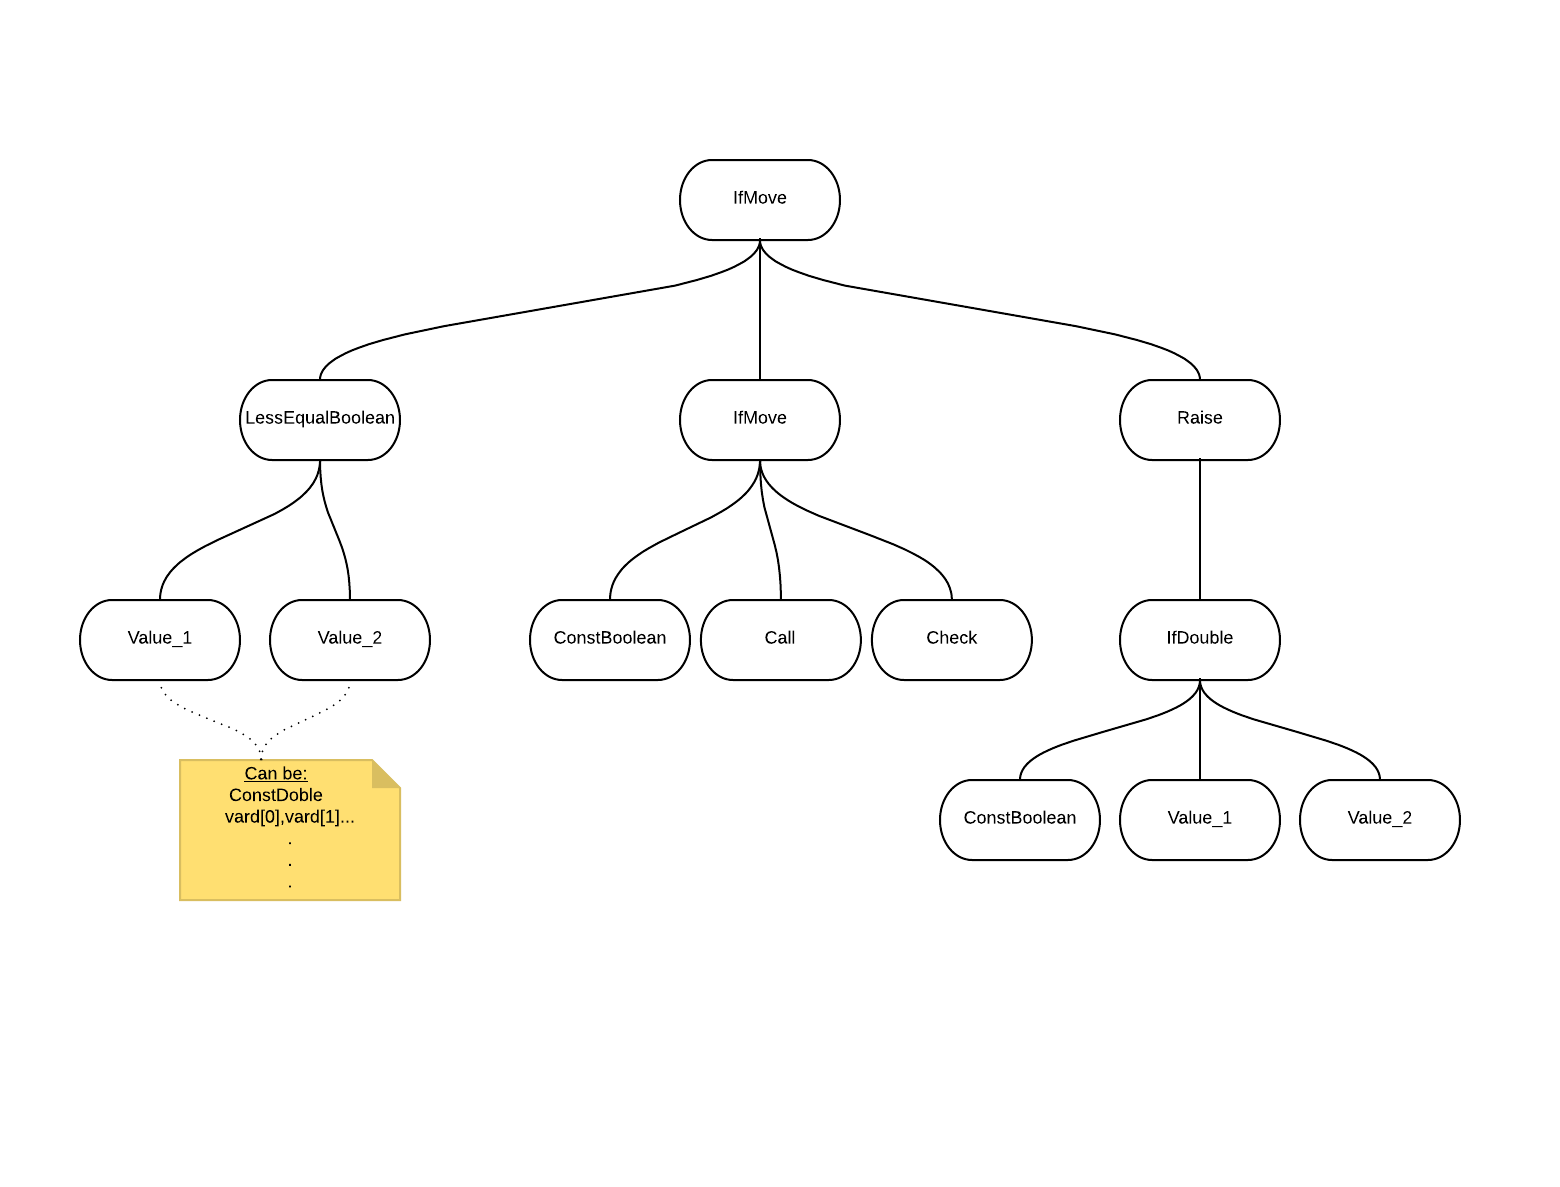
\includegraphics[width=0.95\textwidth]{NewRaise.png}
	\textit{\textbf{Figure 2: }Example tree of an evolved player after the final implementation}
\end{center}

\newpage
\section{Experiments}
For the experiments we evolved two GPlayers both against a "PatternPlayer" and a "TestPlayer" in multiple runs. The first player had the original function- and terminal-set without any additional alterations available. The second player had the aforementioned changes applied. After all test runs were completed, the fitness of the old and new player were compared.

\subsection{Setup}
Nodes used:
\begin{flushleft}
	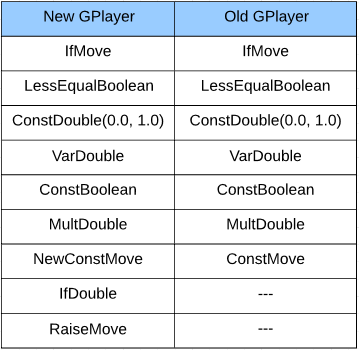
\includegraphics[width=.3\textwidth]{node_table.png}
\end{flushleft}	

\subsubsection{Evolution against PatternPlayer}
The PatternPlayer plays by evaluating his hand value and the overall values of the cards [dividing their rank by an ace and adding them].
The move made depends on their normalized value.

\subsubsection{Evolution against TestPlayer}
One TestPlayer was choosen from previously evolved players that made sane moves and played as follows.
\\
\begin{lstlisting}
	if (getCards().get(1).getRank() < Card.JACK) {
	  if (dealer.getCallBet(this) < 9)
		move.setType(Move.CALL);
	  else
		move.setType(Move.CHECK);
	}else
	  move.setBet((int)(0.9849 * dealer.getPot()));
		
	return move;
\end{lstlisting}

In short, this player was playing more defensively and only performed a "Call" or "Check" when his highest card was lower than a JACK. If his highest card was better he played more aggressively and raised with a value of 0.9849 * pot-size.

\newpage
\subsubsection{Experiment parameter}
For both experiments the parameters were chosen as follows: 
\begin{itemize}
	\item Game Mode:       Doyle
	\item Test-Runs:       8 for each player
	\item Generations:     10.000
	\item Population-Size: 100
	\item Rounds:          1000
	\item Mutation-Rate:   0.0369
\end{itemize} 

A generation of 10.000 seemed to be sufficient for an overall assessment of the fitness. In previous previous test runs using 20.000 generation it was noticed that no best player would emerge after the 10.000th generation.

\subsection{Results}
The following diagrams show the fitness of the old and new player for each run. \\
The fitness is plotted on the y-axis whereas the x-axis displays the number of the run in which the result was recorded. Due to the order the values were recorded in not being in any way relevant the values have been sorted in an ascending order to have a better basis for interpretation. In short, the diagram does not show a function. This needs to be kept in mind when assessing the diagrams.
\subsubsection{Evolution against PatternPlayer}
During evolution against the PatternPlayer it was noted that the changes led to a deterioration of the GPlayer's fitness.  \\ \\
The average calculated fitness of the new GPlayer: 102001\\
The average calculated fitness of the old GPlayer: 113168
\begin{center}
	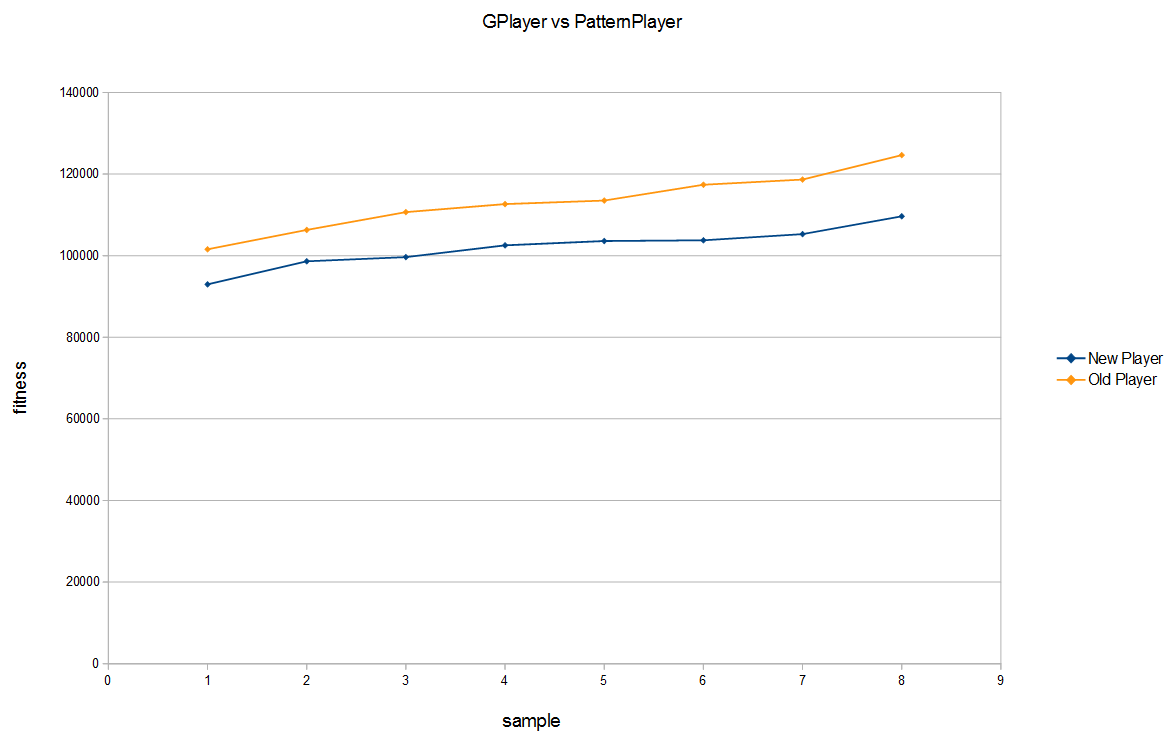
\includegraphics[width=.9\textwidth]{gp_vs_pp_1.png}
\end{center}

\textbf{Evolved trees against the PatternPlayer}\\ 
\texttt{ifm <=d cd[0,8291] cd[0,2086] rcm[Check] rm /d vard[1] *d *d cd[0,5560] cd[0,0537] *d cd[0,0519] cd[0,9908]} \\ \\
\texttt{ifm <=d cd[0,1068] *d cd[0,7747] vard[1] rm cd[0,4432] rm *d vard[0] cd[0,9040]}\\ \\
\texttt{ifm <=d vard[1] *d cd[0.5569] vard[0] ifm <=d cd[0.3677] vard[0] rm *d cd[0.0629] cd[0.1581] ncm[Check] ncm[Call]}\\ \\
\texttt{ifm <=d vard[0] cd[0,6326] ifm <=d vard[1] *d cd[0,3969] vard[0] ncm[Check] ncm[Call] rm cd[0,5256]}\\ \\
\texttt{ifm <=d cd[0,5573] vard[0] rm *d cd[0,7988] *d cd[0,3149] cd[0,3444] ifm <=d *d vard[0] cd[0,5125] vard[1] ncm[Call] ncm[Check]}

\subsubsection{Evolution against TestPlayer}
Overall it is safe to say that the changes improved the performance against the TestPlayer. Although there can be some cases where the old player has a higher fitness than the new one. It was also notable that the overall fitness is cut down to approximately a third compared to the test runs against the PatternPlayer. This is most likely due to the TestPlayer unlike the PatternPlayer making objectively decent moves which results in the GPlayer having a more difficult opponent and hence winning less chips.\\ \\

\section{Conclusion}
Theoretically speaking our alterations provide the player with more information about the current state of the game. This enables the evolution of factors on which the player decides on how high the raise value
shall be. So from a theoretical point of view it is pretty clear that these alterations will lead to the evolution yielding better players. Analyzing our results this assumption can only be confirmed partly. As has been shown the improvement/deterioration is highly dependent on the player against which the GPlayer plays during evolution. This is most likely due to the computer players using different strategies of which one can be easily exploited by the GPlayer using the new function-set whereas the other seems to be more robust. Finally we conclude that although there have been some negative results while playing against the PatternPlayer the result is quite positive. The players emerging after the alterations were made seem to make good decisions and queries (from a poker point of view). Additionally our changes have led to a fairly significant improvement when playing against a player who makes decisions and moves a decent human poker player might make (TestPlayer). 


The average calculated fitness of the new GPlayer: 31153\\
The average calculated fitness of the old GPlayer: 26710

\begin{center}
	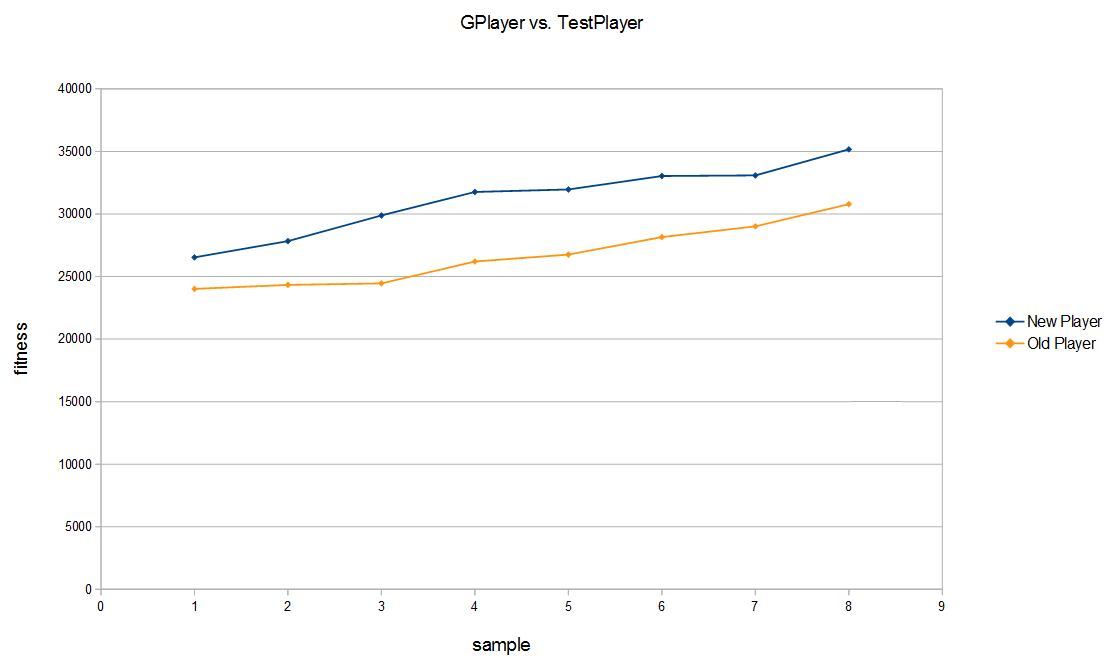
\includegraphics[width=.9\textwidth]{gp_vs_tp_1.png}
\end{center}

\textbf{Evolved trees against the TestPlayer}\\
\texttt{ifm <=d cd[0.5750] vard[0] rm cd[0.3671] ifm <=d vard[0] vard[1] ncm[Call] ncm[Check]} \\ \\
\texttt{ifm <=d cd[0.6027] vard[0] rm cd[0.8510] ifm <=d *d *d vard[0] cd[0.5788] cd[0.9339] vard[1] ncm[Call] ncm[Check]}\\ \\
\texttt{ifm <=d cd[0,1670] *d cd[0,3417] *d cd[0,7303] cd[0,9367] rm cd[0,9624] ncm[Check]}\\ \\
\texttt{ifm <=d cd[0,8291] cd[0,2086] rcm[Check] rm /d vard[1] *d *d cd[0,5560] cd[0,0537] *d cd[0,0519] cd[0,9908]}\\ \\
\texttt{ifm <=d cd[0,4988] /d *d cd[0,2995] cd[0,5651] cd[0,0693] rm /d cd[0,5110] *d *d vard[1] vard[0] ifd cb[false] cd[0,3461] cd[0,5974] rcm[Check]}

\newpage

% links go here, NOT in references

\section{Links}

\begin{itemize}
\item Project Page: \url{https://student.cosy.sbg.ac.at/~tdafir/nc/}
\item PS Page:
\url{http://www.cosy.sbg.ac.at/~helmut/Teaching/NaturalComputation/proseminar.html}

\end{itemize}

\nocite{*}
\bibliographystyle{ieeetr}
\bibliography{report_refs.bib}		% .bib files here

\end{document}
